\documentclass[tikz,border=6pt]{standalone}
\usepackage{amsmath,amssymb}
\usepackage{xcolor}
\definecolor{accent}{HTML}{A13D2C}
\definecolor{accent2}{HTML}{2B5F6B}
\definecolor{muted}{HTML}{5A564F}
\definecolor{linecol}{HTML}{D8D2C4}
\definecolor{astroblue}{HTML}{1B4F72}
\usetikzlibrary{arrows.meta}
\usepackage[T1]{fontenc}\usepackage{newpxtext,newpxmath}  % same fonts as the notes
\begin{document}
% Leading-order chirp of a circular binary, face on (cs:eq:chirp_omega, cs:eq:h0).
% s = (time before coalescence)/(5 G M_chirp/c^3). Orbital angle = s^(5/8) + const, so h_+ = h_0 cos(2 s^(5/8)),
% with h_0 proportional to omega^(2/3), i.e. to s^(-1/4). Plotted from s = 872 (orbital frequency one third of
% the end value) to s = 47, the last stable orbit (r = 6GM/c^2) of an equal-mass pair. Amplitude scaled to 1 there.
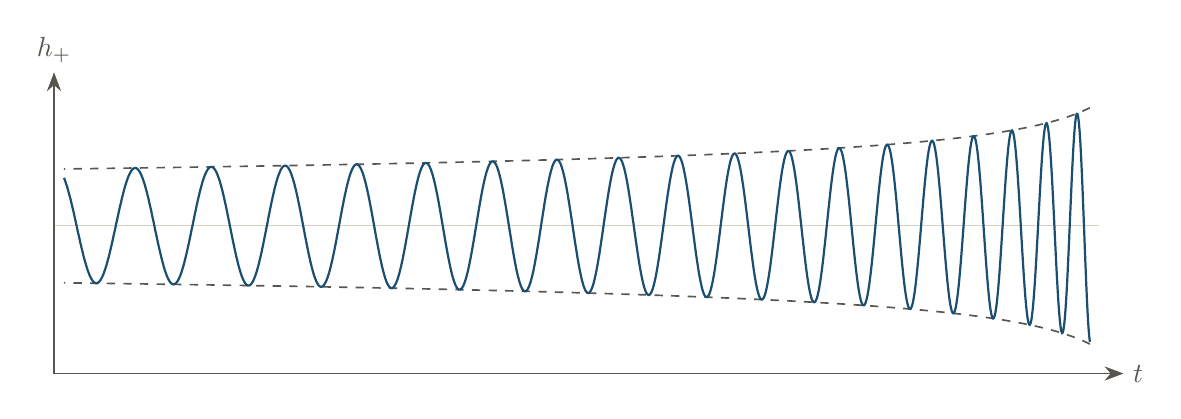
\begin{tikzpicture}[x=0.0158cm, y=1.5cm, >={Stealth[length=2.4mm]}]
  \def\sEnd{47}
  \draw[linecol] (-880,0) -- (-40,0);
  \draw[muted, dashed, line width=0.6pt] plot[domain=\sEnd:872, samples=120] ({-\x}, {pow(\x/\sEnd,-0.25)});
  \draw[muted, dashed, line width=0.6pt] plot[domain=\sEnd:872, samples=120] ({-\x}, {-pow(\x/\sEnd,-0.25)});
  \draw[astroblue, line width=0.8pt] plot[domain=\sEnd:872, samples=1400]
     ({-\x}, {pow(\x/\sEnd,-0.25)*cos(deg(2*pow(\x,0.625)))});
  \draw[->, muted] (-880,-1.25) -- (-20,-1.25) node[right] {$t$};
  \draw[->, muted] (-880,-1.25) -- (-880,1.3) node[above] {$h_+$};
\end{tikzpicture}
\end{document}
